\begin{figure}[H]
    \centering
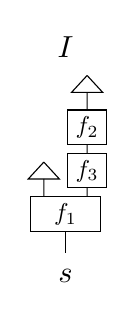
\begin{tikzpicture}[
every node/.style={%
text height=1.5ex,text depth=0.25ex,scale=1.1},scale=1.1]
% Diagram generated by http://github.com/wetneb/MorozParser
\makeatletter


\pgfdeclareshape{triangle}{
    \inheritsavedanchors[from=rectangle]
    \inheritanchorborder[from=rectangle]
    \inheritanchor[from=rectangle]{center}
    \inheritanchor[from=rectangle]{north}
    \inheritanchor[from=rectangle]{south}
    \inheritanchor[from=rectangle]{east}
    \inheritanchor[from=rectangle]{southwest}
    \inheritanchor[from=rectangle]{southeast}

    \backgroundpath{
        \southwest \pgf@xb=\pgf@x \pgf@yb=\pgf@y
        \northeast \pgf@xa=\pgf@x \pgf@ya=\pgf@y
        \pgf@xc=0.5\pgf@xa \advance\pgf@xc by+0.5\pgf@xb

        \pgfpathmoveto{\pgfpoint{\pgf@xc}{\pgf@ya}}
        \pgfpathlineto{\pgfpoint{\pgf@xb}{\pgf@yb}}
        \pgfpathlineto{\pgfpoint{\pgf@xa}{\pgf@yb}}
        \pgfpathlineto{\pgfpoint{\pgf@xc}{\pgf@ya}}
    }
}

\tikzstyle{big-triangle}=[triangle,draw,inner sep=0pt,minimum width=0.5cm,minimum height=0.15cm]
\tikzstyle{medium-triangle}=[big-triangle,scale=0.7]
\tikzstyle{vbig-triangle}=[big-triangle,scale=2]
\tikzstyle{mbig-triangle}=[big-triangle,scale=1.2]
\tikzstyle{small-triangle}=[big-triangle,scale=0.25]
% Curves above:

\node at (0.0,2.6) {$I$};
\node at (0.0,0) {$s$};

\node[rectangle,draw,scale=0.8,minimum width=1cm] at (0,0.7) (fresh) {$f_1$};
\draw (0,0.25) -- (fresh);

\node[medium-triangle] at (0.25,2.2) (td) {};
\draw (td) -- (td |- fresh.north);

\node[rectangle,draw,scale=0.8,minimum width=0.4cm,fill=white] at (0.25,1.2) (n1) {$f_3$};

\node[rectangle,draw,scale=0.8,minimum width=0.4cm,fill=white] at (0.25,1.7) (n2) {$f_2$};
\node[medium-triangle] at (-0.25,1.2) (tg) {};
\draw (tg) -- (tg |- fresh.north);

\end{tikzpicture}

\end{figure}
